%%
%% GMU LaTeX MS Thesis Format Template
%%
%% Developed by:
%%      Daniel O. Awduche and Christopher A. St. Jean
%%      Communications and Networking Lab
%%      Dept. of Electrical and Computer Engineering
%%
%% Notes on usage can be found in the accompanying USAGE_NOTES.txt file.
%%
%%**********************************************************************
%% Legal Notice:
%% This code is offered as-is without any warranty either
%% expressed or implied; without even the implied warranty of
%% MERCHANTABILITY or FITNESS FOR A PARTICULAR PURPOSE!
%% User assumes all risk.
%% In no event shall any contributor to this code be liable for any damages
%% or losses, including, but not limited to, incidental, consequential, or
%% any other damages, resulting from the use or misuse of any information
%% contained here.
%%**********************************************************************
%%
%% $Id: GMU_thesis_template.tex,v 1.16 2007/05/02 02:20:11 Owner Exp $
%%

\documentclass[11 pt]{report}

%%  The file ``gmuthesis.sty''  is the GMU latex style file and
%%   should be placed in the same directory as your LaTeX files
\usepackage{gmuthesis}

%%
%% other packages that need to be loaded, by template
%%
\usepackage{graphicx}                    %   for imported graphics
\usepackage{amsmath}                     %%
\usepackage{amsfonts}                    %%  for AMS mathematics
\usepackage{amssymb}                     %%
\usepackage{amsthm}                      %%
\usepackage[normalem]{ulem}              %   a nice standard underline package
\usepackage[noadjust,verbose,sort]{cite} %   arranges reference citations neatly
\usepackage{setspace}                    %   for line spacing commands

%% The file ``mythesisabbrev.sty'' is an (optional) personalized file that
%% may contain any and all LaTeX command (re)definitions that will be used
%% throughout the document
\usepackage{mythesisabbrev}

\beforedoc

\begin{document}

%% In this section, all of the user-specific fields to be used in the
%% title pages are set
\title{On Privacy in Spatio-Temporal Data:\\User Identification Using Geotagged Social Media}
\onelinetitle{On Privacy in Spatio-Temporal Data: User Identification Using Geotagged Social Media}
\author{Erik Seglem}
\degree{Master of Science}
\subject{Geoinformatics and Geospatial Intelligence}
\doctype{Thesis}
\dept{Geography and GeoInformation Science}

\firstdeg{Bachelor of Arts}
\firstdegschool{American Military University}
\firstdegyear{2014}

\degreeyear{2017}

% Note: semester name should be written in its full-form. For example, Fall Semester, not just Fall.
\degreesemester{Spring Semester}

\advisor{Dr. Andreas Züfle}

\firstmember{Dr. Dieter Pfoser}

\secondmember{Dr. David Wong}

\depthead{Dr. Anthony Stefanidis}

\deanresearch{Dr. Donna M. Fox}

\programdirector{Dr. Peggy Agouris}

%%
%% Introductory pages
%%

% Note: The signature sheet is set according to the requirements of the Volgenau School of
% Information Technology and Engineering. If your college/school requirement is different,
% please make appropriate changes in the "signaturepage" section of gmudissertation.sty file.
\signaturepage

\titlepage

% copyright technically optional but should be included in to avoid potential pagination problems
\copyrightpage

%%
%% Dedication page
%%

\dedicationpage

\noindent I dedicate this thesis to my loving wife, for putting up with all of the time spent on this thesis. Her never ending support was key to its completion.

%%
%% Acknowledgements
%%

\acknowledgementspage

\noindent
I would like to thank the following people who made this possible:
Andreas Z\"ufle, Jan Stutzki, Felix Borutta, Evgheniy Faerman, and Matthias Schubert.

%%
%% Table of contents, list of tables, and lists of figures
%%

\tableofcontents

\listoftables

\listoffigures

%%
%% Abstract
%%
\abstractpage
Trajectory data is among the most sensitive data regarding the privacy of the observed users. To collect trajectory data, mobile phones and other mobile devices constantly track their positions. This work examines the question whether publicly available spatio-temporal user data can be used to link newly observed trajectory data to known user profiles. For this study, publicly available location information about Twitter users is used to construct spatio-temporal user profiles describing a user's movement in space and time. It shows how to use these profiles to match a new trajectory to their user with high accuracy. Furthermore, it shows how to link users of two different trajectory data sets.

For this case study, 15,989 of the most prolific Twitter users in London in 2014 are considered. The experimental results show that the classification approach allows to correctly identify 98~\% of the most prolific 500 of these users. Furthermore, it can correctly identify more than 50~\% of any users by using three locations of these users, rather than their whole trajectory. This alarming result shows that spatio-temporal data is highly discriminative, thus putting the privacy of hundreds of millions of geo-social network users at a risk. It further shows that it can correctly match most users of Instagram to users of Twitter.
\clearpage

%% Be sure to leave a line of whitespace immediately before this line!!!!!
%% (If this comment segment runs together with the preceeding text, you might
%%  see the second page of the abstract numbered "0".)
%%
%% If the abstract is more than one page, then place this line PRECISELY
%% at the page break; otherwise, comment it out.  (See note about this line
%% in the usage notes.)
%%
%%\abstractmultiplepage
%%
%%The second page of the abstract

%%
%%  the main body of the dissertation
%%

\startofchapters

%% include the chapters one by one (or paste the chapter text in directly if desired)
% !TeX root = 00_main.tex

\chapter[Introduction]{Introduction}

It is estimated that a third of the 130 billion copies of applications distributed by Apple's App Store\textsuperscript{\textregistered} access a user's geographic location \cite{appledownloads,appslocation}. As an example, the recently launched augmented reality game ``Pok\'emon Go'', which has been downloaded more than 100 million times on Android devices alone \cite{pokemongo}, constantly synchronizes the GPS location of users with a company server. While users trust that their location data will be used in sensitive fashion, Apple\textregistered{} recently updated its privacy policy to allow sharing the spatio-temporal location of their users with ``partners and licensees''\cite{appleprivacy}.

The mobility behavior of a person often reveals a large variety of sensitive information, which they may not be aware of.
A list of potentially sensitive professional and personal information that could be inferred about an individual, knowing only their mobility trace, was published recently by the Electronic Frontier Foundation \cite{Blumberg2009}. Such personal information could simply be marketing information, obtained from a user's choice of restaurants, or a user's religious beliefs, inferred through the proximity to a particular church. It can also indicate other, much more sensitive, information about an individual based on their presence in a motel or at a medical clinic.

\begin{figure}[p]
	\centering
	\begin{subfigure}[b]{\textwidth}
		\centering
		\includegraphics[width = 0.7\textwidth]{figures/1_user_12_week_small.png}
		\subcaption{Weekly history of a single user.}
    \label{fig:intro:1user}
  \end{subfigure}

	\begin{subfigure}[b]{\textwidth}
		\centering
		\includegraphics[width = 0.7\columnwidth]{figures/10_user_12_week_2-0_small.png}
		\subcaption{12-week trajectory of 10 users.}
    \label{fig:intro:10user}
	\end{subfigure}
  \caption{Illustration of Twitter Trajectories}\vspace{-0.0cm}
  \label{fig:exsinglefit}
	\figSpace
\end{figure}

In this work, the severity of privacy risks through publishing individual spatio-temporal data on the use case of Twitter data is investigated. In particular, it is shown that geotagged tweets might yield enough location information for building user specific trajectory profiles. Based on these profiles, Twitter accounts can be linked to additional trajectory data being observed from unknown users. Other location based services or mobile devices are also potential sources for trajectories. Additionally, face detection methods tag known persons in images in social networks. Thus, geotagged images can reveal a user's whereabouts at certain points in time. Given that there are multiple such images, it might be possible to build a trajectory and link it to a known user. To conclude, freely available location data might be used to link accounts and devices for the same user. Thus, the user reveals more of his movements and actions than might be intended.

To derive trajectory profiles for a given Twitter account, geotagged tweets containing an exact geolocation, a time, and a user ID were collected. Since this work focuses on the location aspect the content of the Tweet is completely ignored, even though it might add even more useful information to user profile. Using the Twitter API, or similar micro-blogging applications, users can publish a short text message, called a Tweet, together with their current geolocation, a current time-stamp, and their user ID.

The sequence of Tweets of a user is interpreted as a trajectory. For each user, all available Twitter data is used to build a trajectory profile to capture each user's specific mobility patterns. Using these profiles, new trajectories, for which the originating user is unknown, can be linked to a known user with an alarmingly high accuracy. To illustrate this classification problem, a typical Twitter trajectory of a single user is depicted in Figure \ref{fig:intro:1user}. The figure shows a twelve week trace of a user's tweets, in color-coded one-week intervals. For comparison, Figure \ref{fig:intro:10user} shows the same twelve week traces for ten users, using a different color per user. Note that the tweets of this user are voluntarily published by the user, such that Figure \ref{fig:intro:1user} and Figure \ref{fig:intro:10user} do not raise any privacy concerns.

The challenge of this work is to match a new short trajectory, such as a one week trajectory corresponding to a single color in Figure \ref{fig:intro:1user}, to the correct user corresponding to one of the colors in Figure \ref{fig:intro:10user}. Note that the ten selected user profiles in the example are located in  relatively distinct activity regions. Thus, finding the right profile is relatively simple. In a more realistic setting, distinguishing thousands of users in the same area, and user identification is significantly more challenging. In these experiments up to 15,989 users, within the same bounding box of London, are used leading to a much more challenging classification task.

Twitter data is comparatively sparse to other location tracking applications, as tweets are typically published at a frequency of less than one per hour. Despite this data sparsity, it is shown that a large quantity of low-quality location data can still be used to construct highly discriminative user models. To summarize the contributions of this work are as follows:

\begin{itemize}
	\item Trajectory models to capture user-specific movement profiles from sparse trajectories obtained from Twitter.
	\item Methods for mapping a newly observed trajectory of an unknown user to the most likely user in the database.
	\item An experimental evaluation showing that individual patterns are highly unique and allow for a user classification accuracy of up to 98\% .
	\item A case study of linking users of Twitter to users of Instagram, with an accuracy of up to $81\%$.
\end{itemize}

The remainder of this paper is organized as follows. Chapter~\ref{sec:rw} describes
related work of analyzing trajectory data and user identification. In Chapter~\ref{sec:probdef}, problem setting is formalized and the task of linking new trajectories to users is definied. Chapter~\ref{sec:method} describes the trajectory models and the approach to user identification. The results of the experimental evaluation are described in Chapter~\ref{sec:experiments}. Scalability of this solution is address in Chapter~\ref{sec:scalability} and further user linkage experiments are address in Chapter~\ref{sec:linkage}. It is concluded in Chapter~\ref{sec:conclusion}, with additional research opportunities addressed in Chapter~\ref{sec:additional}.

% !TeX root = 00_main.tex

\chapter[Related Work]{Related Work}
\label{sec:rw}
This section provides a survey of the state-of-the-art in spatio-temporal user identification, trajectory based user linkage, and trajectory privacy. User identification is focused on identifying the same user again within the same database, while user linkage is focused on linking two users together across multiple sources of data. This work assumes that user trajectory data is fully available, without any notion of privacy preservation. This assumption is appropriate in the experimental evaluation, using publicly available Twitter data. However, other trajectory data sets may employ some form of privacy, thus it is important to understand privacy methods, which might be used on trajectory data.

\section{User Identification}
A problem similar to the problem of trajectory based user-identification was considered in \citeauthor{DeMontjoye2013} \cite{DeMontjoye2013}. This work estimates the number of points needed to uniquely identify an individual trajectory. The dataset contained 15 months of data on ~1.5M users in a small European country. Each time a user connected to a mobile phone tower to send or receive a call or text message, a tower location and time, with a resolution of one hour, was recorded. There are almost 6500 unique antennas in the dataset, and on average each user has 114 interactions per month. Among this dataset, they found that four randomly chosen points of a trajectory were enough to uniquely identify 95\% of the trajectories, and two randomly chosen points were enough to identify 50\% of the trajectories. However, the question whether a trajectory is unique, is different to the problem of user-identification tackled in this work.

The user-identification method in \citeauthor{DeMontjoye2013} assumes that a trajectory of the user to be identified is already in the database. Thus, a new trajectory, which has not been seen before, cannot be classified. Summarizing, the work in \citeauthor{DeMontjoye2013}, aims at identifying individual trajectories, rather than individual users. Their work provided an initial framework to build this work on.

The work presented in \citeauthor{Bettini2005} \cite{Bettini2005} investigates the problem of how to prevent the identification of actual persons behind the users of location based services. Therefore, the authors employ so-called location-based quasi identifiers, which are formed from historical spatio-temporal movement patterns that are gathered from location-based service requests as a potential privacy concern. However, the stated problem is slightly different from this work, as they make use of external sources to finally get the real names behind the pseudonames.

\section{User Linkage}
There are a variety of publications considering the problem of user linkage or more general record linkage. In the database community, record linkage generally aims at detecting duplicate records within one or several databases. Records describing the same entity may not share a common key or contain faulty attribute values, which makes the detection of such duplicates non-trivial. A survey on the proposed approaches can be found in \citeauthor{Elmagarmid2007} \cite{Elmagarmid2007}.

Considering networks, record linkage is widely understood as user linkage and is stated as the problem of linking corresponding identities from different communities appearing within one or many networks \citeauthor{Zafarani2009} \cite{Zafarani2009}. It is specifically tailored to the requirements of user identification in heterogeneous data by considering co-occurrences adjusted with a stimulus signal. The stimulus signal is derived from locations with frequent co-occurrences and decays with increasing distance to a trajectory. The stimulus signal allows this method to weight important locations, which helps to distinguish two users with very similar trajectories.

An important area of user linkage is social networks where the user linking problem aims at connecting user profiles from different platforms that are used by the same persons. \citeauthor{Liu2013} \cite{Liu2013} differentiate between three types of user linkage across social networks: user-profile-based methods, which use information provided by the profiles to connect corresponding profiles \cite{Malhotra2012}, user-generated-content-based approaches, which analyze the content published by the users to link profiles \cite{Liu2013} and user-behavior-model-based methods that generate models based on the (temporal) user behaviors and finally link user profiles based on the similarity of these models \cite{Liu2014}.

Most related to this approach is the recent work of \citeauthor{Cao2016} \cite{Cao2016}. In this work, the authors use various sources for the trajectories and propose a MapReduce-based framework called Automatic User Identification (AUI). They identify sample rate, temporal and spatial sparsity and the fact that people with a close relationship provide similar trajectories as distinct features of the data. Sparsity of the data is corrected by using a long time frame. Signal Based Similarity (SIG) is introduced as a measurement of the similarity of two trajectories. In contrast to that approach, this work uses sparser trajectories. While the authors of \citeauthor{Cao2016} do consider sparse social media data, they accumulate these trajectories during a long time interval of at least multiple months. In this work, a long term mobility history of user is not assumed to be  available. Instead, it aims at identifying users with as few observations as possible.

\section{Trajectory Privacy}
The predominantly used measurement for privacy is k-anonymity \cite{Sweeney2002}, which works with a closed world assumption and assures that, for each query that could be used to identify the identity of a user, at least $k-1$ other users are returned as possible results.

Common approaches to guarantee a defined degree of anonymity are suppression, obfuscation and generalization \cite{Hashem2007}. To achieve k-anonymity by suppression, every element that does not fit into an anonymity set is removed \cite{Byun2007, Lefevre2006}. For trajectories, oppression would require discarding observations in discriminative locations such as a user's home. While this method is effective, the use of only suppression can lead to a significant loss of information. Perturbation is another method used to obfuscate the data \cite{Aggarwal2004}. The goal is to generate a synthetic dataset with the same properties of the original dataset using a generative model. For generalization, $k$-groups of users could simply be unified into a single entity.

This work does not try to maintain privacy of users, and can be seen as an adversary approach of trying to breach the privacy of users. A highly relevant future piece of work is to investigate how existing privacy preservation methods for trajectories can be employed to suppress, obfuscate and generalize trajectories to minimize the user identification accuracy of this solutions, while further minimizing the loss of information in the data.

A more refined version of k-anonymity is l-diversity, which addresses some shortcomings of k-anonymity \cite{Machanavajjhala2006}, mainly where properties of the data are homogeneous and allow conclusions, which might violate the assured k-anonymity. Regarding trajectories, location l-diversity is required as introduced in \citeauthor{Beresford2003} \cite{Beresford2003}. As an enhancement of l-diversity, t-closeness \cite{Li2007} is used on datasets where the distribution of attribute values allows conclusions to identities.

These measurements are typically applied when medical records are published or in regards to Location Based Services (LBS), which require personalized location information. As LBS are usually working with GPS coordinates and trajectories, the raw data is similar to the information. But there is a difference in quality and frequency. LBS usually work with the assumption that a user is willingly providing her location as precise as possible and/or performing measurements of the location with a high frequency. While work has been done on interpolating real trajectories from purposefully obfuscated ones \cite{Naghizade2015}, the data used is limited to one service and focusing on the k of k-anonymity instead on user identification.

The work of \citeauthor{Abul2008} \cite{Abul2008} applies k-anonymity on spatio-temporal objects introducing the $(k, \delta)$-anonymity. The trajectories of a user are extended by the uncertainty of the location measurement $\delta$. The authors claim that a series of trajectories and locations can be modeled as a series of cylinders, or a tube. k-anonymity is granted when $k-1$ additional elements of the set can fit into a tube. The proposed method uses outlier detection and other forms of suppression in combination with space transformation of a maximum of $\delta/2$ while $\delta$ defining the circumference of the tube remains unchanged. The paper proposes a heuristic that succeeds to find anonymity sets as the problem is NP-hard.

The notion of $(k, \delta)$-anonymity is also discussed in \citeauthor{Trujillo-Rasua2013} \cite{Trujillo-Rasua2013}. The authors come to the conclusion
 that existing methods to create $(k, \delta)$-anonymity as developed in \citeauthor{Abul2008} are not sufficient if $\delta > 0$. By defining every location in a spatio-temporal trajectory as a quasi-identifier and assuming that a potential adversary has knowledge about one sub trajectory they show that the probability to correctly identify a series of trajectories is larger than $1/k$ thus violating the $k$-anonymity. This work will show that it is indeed possible to identify users with high probability by only knowing a sub trajectory.

% !TeX root = 00_main.tex

\chapter[Problem Definition]{Problem Definition}
\label{sec:probdef}
In this work, the question of to what extent a set of spatio-temporal observations, such as geotagged tweets, are sufficient to derive spatial user profiles for the observed users and reliably link spatial trajectories of unknown users to one of the known user profiles is answered. Therefore, this section will define terms and notations, and formally define the problem of user identification using trajectory data.

In this paper, spatio-temporal data is considered. That is data of users annotated with a geolocation and a timestamp, such as obtained from Twitter.
\begin{definition}[Spatio-Temporal Database]
Let $\mathcal{U}$ denote a set of unique user identifiers, let $\mathcal{S}$ be a set of spatial regions, and let $\mathcal{T}$ denote a time domain.
A \emph{spatio-temporal database} $\DB\subseteq \mathcal{U}\times \mathcal{S}\times \mathcal{T}$ is a collection of triples $(id\in\mathcal{U},s\in\mathcal{S},t\in\mathcal{T})$. Each triple $(u,s,t)\in\DB$ is called an observation.
\end{definition}
Furthermore, a trajectory is defined as a sequence of location and time pairs.
\begin{definition}[Trajectory]
A trajectory $tr\subseteq \mathcal{S}\times\mathcal{T}$ is a collection of pairs $(s\in\mathcal{S},t\in\mathcal{T})$.
\end{definition}

To build a user specific mobility pattern, the data is temporally partitioned $\DB$ into equal sized time intervals called epochs. For each epoch, the set of observations of a specific user is called a trajectory, formally defined as follows.
\begin{definition}[Database Trajectories]
Let $\DB$ be a spatio-temporal database. Let $\mathcal{E}=\{e_1,...e_n\}$ be a partitioning of $\mathcal{T}$ into $n$ temporal intervals denoted as epochs. For each epoch $e\in\mathcal{E}$, and each user $u$, the trajectory
$$
\DB(u,e):=\{(u^\prime,s,t)\in\DB|u^\prime=u, t\in e\},
$$
is called the database trajectory of user $id$ during epoch $e$.
\end{definition}


In the remainder of this paper, trajectory models are introduced to capture the motion of a user in space and time. The models are derived from the set of all trajectories of a user, called their trajectory profile formally defined as follows.
\begin{definition}[Trajectory Profile]
Let $\DB$ be a spatio-temporal database, let $u\in\mathcal{U}$ be a user and let $\mathcal{E}$ be a temporal partitioning of $\DB$ into $n$ epochs.
The trajectory profile $\mathcal{P}(u)$ the set of all trajectories of $u$, i.e.,
$$
\mathcal{P}(u)=\{D(u^\prime,e)|u^\prime=u,e\in\mathcal{E}\}.
$$
\end{definition}
The main challenge of this paper is to identify the trajectory of an unknown user.
\begin{definition}[User Identification]
Let $\DB$ be a spatio-temporal database and let $Q\subseteq \mathcal{S}\times\mathcal{T}$ be a trajectory of an unknown user $x$. The task of user identification is to predict the unknown user $u$ of $Q$ given $\DB$. The function
$$
\mathcal{I}:\mathcal{P}(\mathcal{S}\times\mathcal{T})\mapsto \mathcal{U},
$$
maps a trajectory $Q$ to user $x$ as a user identification function.
\end{definition}
Thus, user identification is a classification task mapping a trajectory to its unknown user.
To train a user identification function $I(Q)$, the next section presents the classification approach, which uses the trajectories in $\DB$ as a training set, in order to predict the user of a new trajectory $Q\notin\DB$.

% !TeX root = 00_main.tex

\chapter{Trajectory based user identification}
\label{sec:method}

Trajectory models are introduced to capture the motion of a user $u\in\mathcal{U}$ in space and time by learning from their trajectory profile $\mathcal{P}(u)$ in Subsection \ref{subsec:modeling}. For each model, a similarity measure to quantify similarity between different trajectory models is proposed. Based on these similarity measures, the user identification approach is presented in Subsection \ref{subsec:class}. As mentioned before, the prediction is based on the assumption that there exists a profile $P(u_i)$ for each user $u_i \in U$.

\section{Trajectory Profile Modeling}\label{subsec:modeling}
Each trajectory $\mathcal{\DB}(u, e)$ of user $u$ during epoch $e$ is a sequence of observations, i.e., time-stamped geo-locations. A spatial grid to partition geo-space into equal sized regions $\mathcal{S}=\{S_1,S_{|S|}\}$ is used, thus reducing a trajectory to a sequence of time-stamped grid-cells. To model such a sequence, two kinds of approaches are proposed:
\begin{itemize}
\item The first approach using \emph{set descriptors} treats a trajectory as a \emph{set} of grid-cell observations, thus ignoring the sequence, ordering, and time-stamps of these observations.
\item The second approach using \emph{frequent transitions} considers the transitions of users from one spatial region to another, thus explicitly modeling the order of observations.
\end{itemize}

\subsection{Set Descriptors}\label{subsubsec:set}
Ignoring the temporal aspect, a trajectory $\DB(u, e)$ of user $u$ during epoch $e$ can be described by a vector $v(u,e)$ all spatial regions in $S$. In other words, each spatial region is represented by a dimension of $v(u,e)$.

Note that $v(u,e)$ contains zero values in the majority of dimensions as each user usually only traverses a small fraction of space during an epoch. In other words, $v(u,e)$ is sparse.
Modeling trajectories using frequency descriptions has a strong resemblance to handling bag of words vectors known in text mining. To describe, if and how often a domain was visited within trajectory $\DB(u,e)$, the following two approaches are examined.

Simple examples of these can be seen in Figure \ref{fig:trajectory_creation}. Each color represents different users geotagging in the area of interest. Then a 4x4 grid is applied to the area, and set descriptors are generated from the data.

\begin{figure}[ph]
	\centering
	\begin{subfigure}[b]{\textwidth}
		\centering
		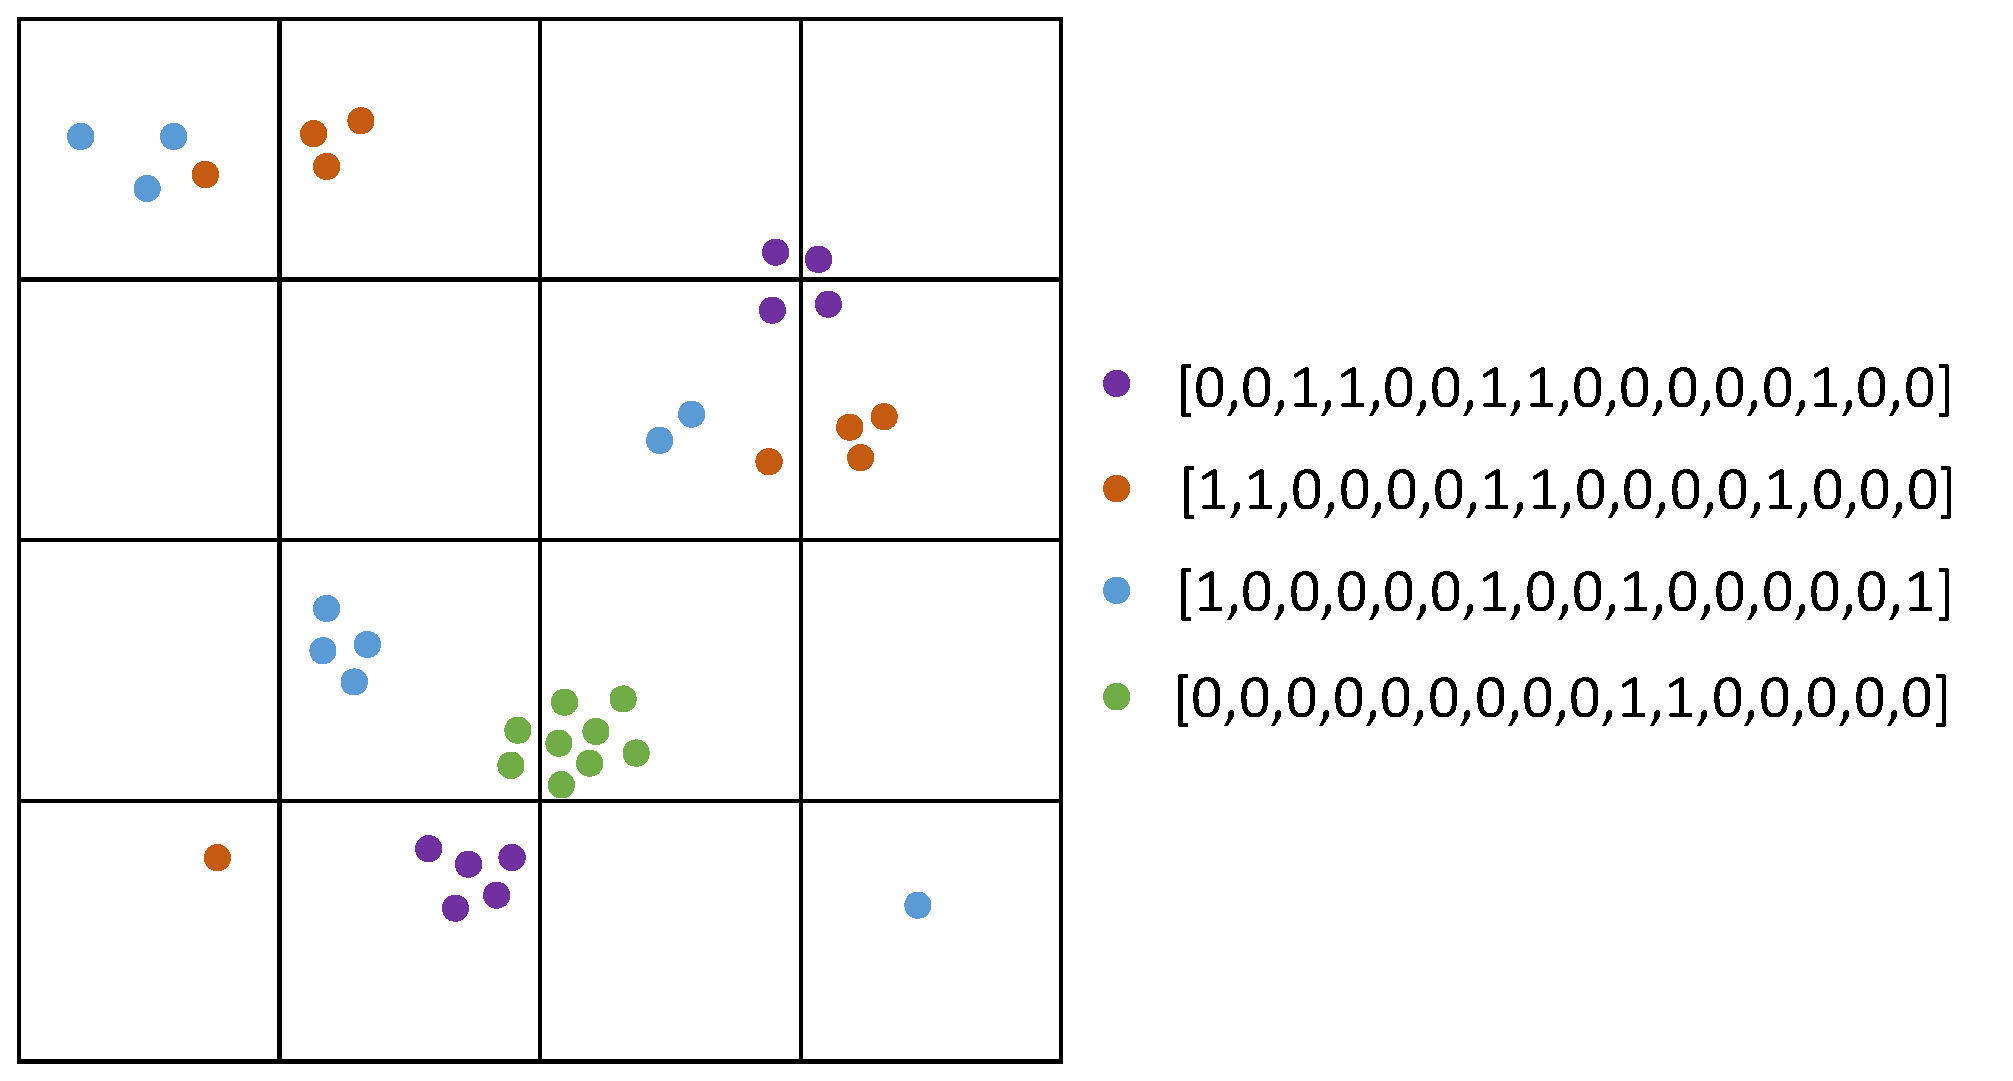
\includegraphics[width = 0.9\textwidth]{figures/trajectory_bitset}
		\subcaption{Bitset Descriptor}
    \label{fig:trajectory_bitset}
	\end{subfigure}

	\begin{subfigure}[b]{\textwidth}
		\centering
		\includegraphics[width = 0.9\textwidth]{figures/trajectory_frequency}
		\subcaption{Frequency Descriptor}
  	\label{fig:trajectory_frequency}
	\end{subfigure}
  \caption{Set descriptor trajectory creation.}
  \label{fig:trajectory_creation}
	\figSpace
\end{figure}

\paragraph{Bitset Descriptor}
In this rather simple method, a trajectory $\DB(u,e)$ is represented as a set of visited spatial regions. Thus, each feature value $v^{\mbox{bit}}$ equals one if user $u$ visited region $S_i$ (at least once) during epoch $e$, formally:
$$
v^{\mbox{bit}}_i (u,e):=
\begin{cases}
        1,& \text{if }\exists (u^\prime,s,t)\in\DB: u^\prime=u \wedge s\in S_i \wedge t\in e,\\
        0, & \text{otherwise}
        \end{cases}
$$
A visual example of this is shown in \ref{fig:trajectory_bitset}.

To compare bitset vectors $v, v^\prime  \in \{0,1\}^n$, the Jaccard coefficient is employed, which is a standard similarity measure for sets:
\begin{definition}[Jaccard Coefficient]
Let $v,v^\prime \in \{0,1\}^n$ be two bit vectors, then the Jaccard coefficient is defined as follows:
\begin{displaymath}
Jac(v,v^\prime)=\frac{\sum_{i=1}^n v_i \wedge v_i^\prime}{\sum_{i=1}^n v_i \vee v_i^\prime}
\end{displaymath}
\end{definition}

\paragraph{Frequency Descriptors}
A frequency vector $v^{\mbox{freq}}$ contains the number of visits of each spatial region of user $u$ in epoch $e$. This allows to distinguish between users visiting a particular region more or less often than other users.
$$
v^{\mbox{freq}}(u,e)_i=|\{(u^\prime,s,t)\in\DB|u^\prime=u \wedge s\in S_i \wedge t\in e\}|.
$$
A visual example of this is shown in \ref{fig:trajectory_frequency}.

The standard way to compute the similarity in sparse numerical vectors is the cosine coefficient:
\begin{definition}[Cosine Coefficient]
Let $v,v^\prime \in \NN^n$ be two vectors, then the Cosine coefficient is defined as follows:
\begin{displaymath}
Cos(v,v^\prime)=\frac{v^T \cdot v^\prime}{||v|| \cdot ||v^\prime||}
\end{displaymath}
\end{definition}
Since the cosine coefficient can be strongly dominated by dimensions having high average frequency values, spatial regions are normalized by their total number of observations.

\subsection{Transition Descriptors}\label{subsubsec:trans}
All of the previous trajectory descriptors had in common that they treat a trajectory as an unordered set of locations, without considering any notion of sequence or time. In this section, a trajectory is treaded as a sequence of regions. As a baseline to compute the similarity between two sequences, dynamic time-warping \cite{Berndt1994} (DTW), a state-of-the-art method for similarity search on sequences, is used. Since the experimental evaluation shows that using DTW without any adaption as a similarity measure yields a fairly low classification accuracy, this section presents two approaches to directly model the transitions of a trajectory. A transition is a pair $(s,s^\prime)$ of regions where $s$ is called source and $s^\prime$ is called destination. Using a descriptor for each pair of spatial regions $s_i,s_j$, describing the number of times the specific sequence $(s_i,s_j)$ has been observed in a trajectory $\DB(u,e)$, is proposed.

\begin{definition}[Trajectory Transitions]
Let $\DB(u,e)=\{(s_1,t_1),...,(s_n,t_n))\}$ be a trajectory, the set of transitions $\uparrow\DB(u,e)$ is defined as the multi-set (thus allowing duplicates)
$$
\uparrow\DB(u,e):=\bigvee_{1\leq i< n}(s_i,s_{i+1}).
$$
The number of occurrences of $(s,s^\prime)$ in trajectory $\DB(s,e)$ is denoted as $\uparrow\DB(u,e)(s,s^\prime)$.
\end{definition}
Since modeling all observed transitions blows up the feature space quadratically, Using only the $k$ globally most frequent transitions as features is proposed.
\begin{itemize}
  \item {\bf Frequent Transitions:} The globally most frequent transitions are searched for and the number of occurrences of these transitions is used as a feature vector to describe a trajectory.
  \item {\bf Transition Probabilities:} Common transitions of two trajectories are found, and their similarities are adapted by the global rarity of these transitions.
\end{itemize}

\begin{definition}[Top-$k$ Most Frequent Transitions]
Let $k$ be a positive integer, then the set $FT$ is a set of pairs of spatial regions defined as
$$
FT^k(\DB)=argmax^k_{s_i,s_j\in \mathcal{S}} |\{\sum_{u\in\mathcal{U},e\in\mathcal{E}}\uparrow\DB(u,e)(s_i,s_j)\}|,
$$
where $argmax^k_X(\varphi)$ returns the set of $k$ arguments $x\in y$ yielding the maximum value substituted in term $\varphi$.
\end{definition}
Now the $k$ most frequent transitions $FT^k(\DB)$ can be used as additional features.
Similar to the set descriptors presented in Subsection \ref{subsubsec:set}, the features are described using
\begin{itemize}
\item Bit vectors, using the feature vector
$$
v^{\uparrow\mbox{bit}(u,e)}_i=\begin{cases}1 & \text{if }FT^k(\DB)_i\in \uparrow\DB(u,e) \\ 0 & \text{otherwise}\end{cases}
$$
\item Frequency vectors, using the feature vector
$$
v^{\uparrow\mbox{freq}}(u,e)_i=\uparrow\DB(u,e)(FT^k(\DB)_i)
$$

\end{itemize}
For these vectors, the same similarity functions defined in Section \ref{subsubsec:set} can be used.

\section{Classification}\label{subsec:class}
Regardless of which of the modeling approaches presented in this section is employed, the result is a high-dimensional feature vector. To classify a new trajectory of an unknown user, the next section proposes the classification procedure, using the previously proposed user-specific trajectory models. To classify the user of a new trajectory, a $k$-nearest neighbor classification approach is employed. This choice is made due to the extremely high dimensional feature space, having one dimension per spatial grid-cell.
Therefore, given a trajectory database $\DB$, trajectories $\DB(u,e)$ are extracted for each user $u$ in each epoch $e$. Since the user is known for each of these trajectories, the result is a labeled dataset $P_{train}$ of feature vectors. Given a new trajectory $Q$, map $Q$ to its feature description $v_{new}$ and search the $k$-nearest neighbors of $v_{new}$ in $P_{train}$ w.r.t. a corresponding similarity measure. To decide the final class decision, each queried neighbor is weighted by its similarity value and the class is predicted as the one having the largest cumulated similarity.

Formally, this can be define the $k$-nearest neighbors classification as follows.
Let $P_{train} = \lbrace (v_i, y_i)~\vert~v_i \in \lbrace 0, 1\rbrace ^n \wedge y_i \in \mathcal{L} \rbrace$ be the set of training instances consisting of pairs $(v_i, y_i)$ with $v_i$ being the feature description of the user trajectory $i$ and $y_i$ being the label, i.e., identity of the user, assigned to trajectory $i$. $\mathcal{L}$ denotes the set of labels.
Given the feature description $v_{new}$ of a query trajectory, the identity, resp. label, $y_{new}$ of $v_{new}$ is determined by cumulating the similarities, i.e., $d(.,.)$, for each label $l \in \mathcal{L}$ represented among the $k$-nearest neighbors of $v_{new}$ and taking the most representative label.
$$y_{new} = argmax_{l \in \mathcal{L}} \lbrace \sum{d(v_{new}, v_k^l)}~\vert~v_k^l \in kNN(v_{new}) \rbrace$$
Note that no index structure is used to support the $k$NN-search due to the high dimensionality of the feature space.

\section{User Linkage}\label{subsec:linkage}
In addition to the identification of individual users, another application of the user trajectory profiling is to link users between two trajectory datasets. Therefore, let $\DB$ and $\DB^\prime$ be two trajectory databases having the set of users $\mathcal{U}$ and $\mathcal{U}^\prime$, respectively. The task of user linkage is to find pairs of database users $(u\in\mathcal{U},u^\prime\in\mathcal{U}^\prime)$ that correspond to the same individual in the real world, i.e., having $u=u^\prime$. As an example, the two data sets may correspond to Twitter and Instagram. The same individual may have different user names in both social networks. The task of user linkage is to find such individuals.

Clearly, using the approach presented in Section \ref{subsec:class}, the trajectories of each user are classified in $\DB$, and the most similar user in $\DB^\prime$ is classified. The drawback of such approach is that multiple users in $\DB$ may be matched to the same user in $\DB^\prime$, and some users in $\DB\prime$ might not have any match. To avoid this drawback, the matching problem is formalized as a bipartite graph, containing for each $(u\in\mathcal{U},u^\prime\in\mathcal{U}^\prime)$ a weight of similarity. This similarity is chosen by performing a $k$NN search of each trajectory in $\DB$ on the database $\DB^\prime$. Then, the score of $(u,u^\prime)$ corresponds to the number of occurrences of $u\prime$ in $k$NN sets of all trajectories of user $u$.

Given this bipartite graph, the Hopcroft-Karp algorithm \cite{Hopcroft1973} is used to find an optimal matching, i.e., mapping of each user in the smaller database to exactly one user in the other that maximizes the total score.

% !TeX root = 00_main.tex

\chapter[Experimental Evaluation]{Experimental Evaluation}
\label{sec:experiments}

The proposed approach is evaluated on a dataset mined from Twitter using their public API, feeding from a global $1\%$-sample over the time interval from December 30, 2013 to March 24, 2014, using a $(51.25,51.75)$ degrees longitude to $(-0.55,0.30)$ degrees latitude window covering the London region shown in Figure \ref{fig:intro:10user}.

\begin{figure}[ph]
	\centering
	\begin{subfigure}[b]{\textwidth}
		\centering
		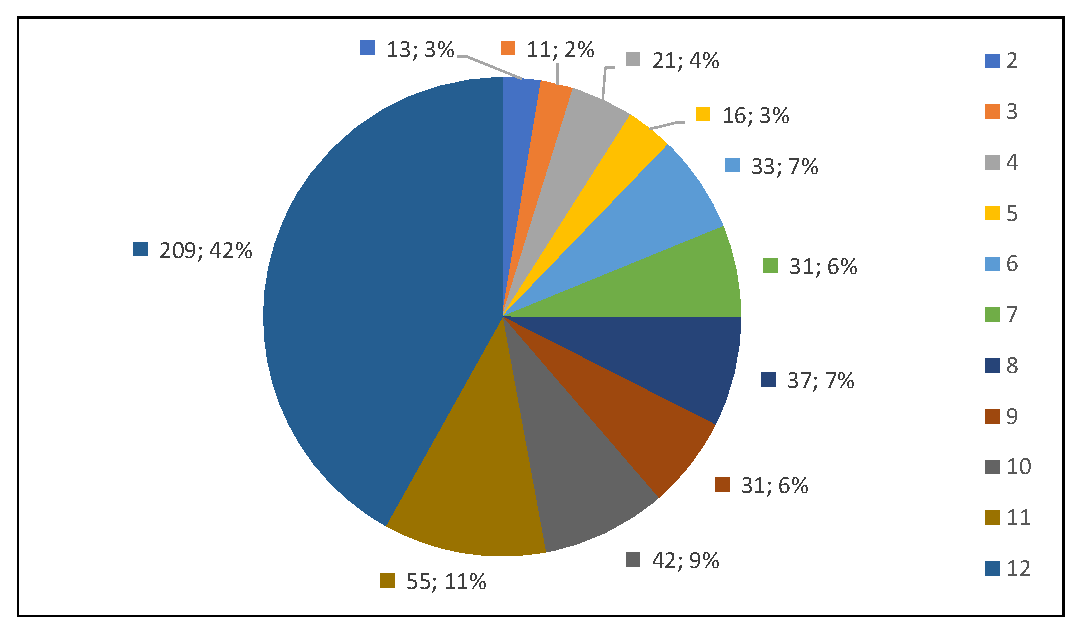
\includegraphics[width = 0.8\textwidth]{figures/500_trajectories_per_user}
    \subcaption{Trajectories within the 12 epochs}
    \label{fig:500_traj}
	\end{subfigure}

	\begin{subfigure}[b]{\textwidth}
		\centering
		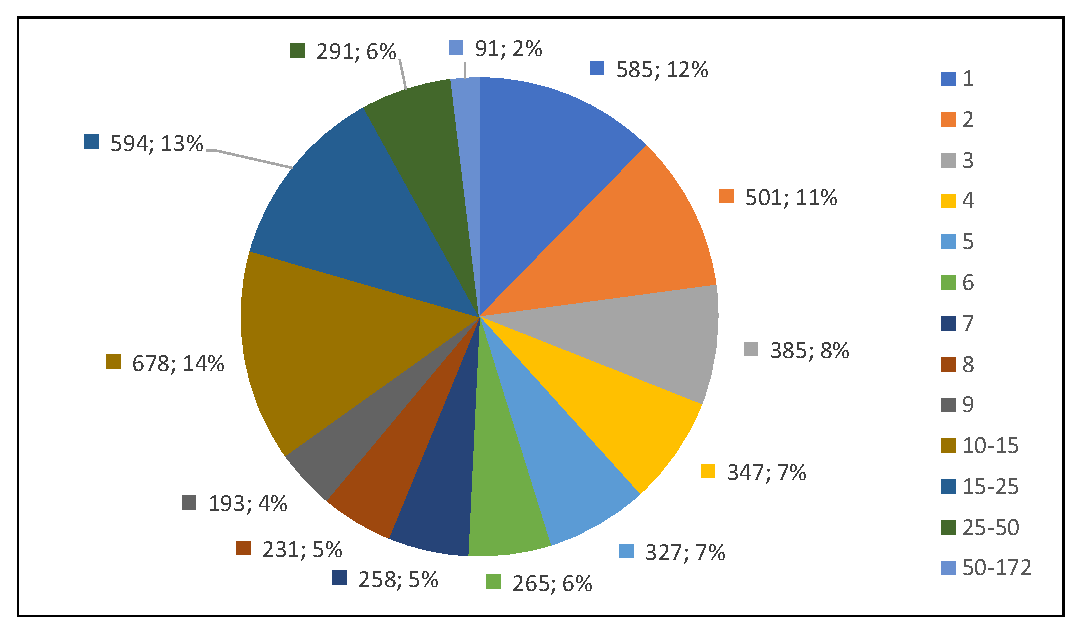
\includegraphics[width = 0.8\textwidth]{figures/500_observations_per_trajectory}
		\subcaption{Observations per one-week Trajectory}
    \label{fig:500_obs}
	\end{subfigure}
  \caption{Distribution of the Top 500 most prolific users in the London-Twitter Dataset.}\vspace{-0.2cm}
  \label{fig:500_dist}
	\figSpace
\end{figure}

Out of these London-Tweets, the top-500 most prolific users were selected, excluding obvious spammer or bot users. This dataset is split into temporal epochs of one-week. Thus, the database contains a total of $|\mathcal{U}|=500$ users, and a total of $|\mathcal{E}|=12$ epochs. Consequently, the database $\DB$ contains a total of $\mathcal{U}\times\mathcal{E}=6000$ trajectories.

To discretize space, a spatial grid is applied on the aforementioned rectangle covering the London region, having an extent $ext$ in longitude and latitude ranging from $0.01'$ to $0.001'$. The set of all resulting grid cells constitutes the set of spatial regions $\mathcal{S}$, having $|\mathcal{S}|=4.250$ cells for $ext=0.01'$ and $425.000$ cells for $ext=0.001'$. Table \ref{} shows all grid sizes as well as the dimensions of the related trajectories.

\begin{table}
  \centering
  \caption{Grid Sizes and Total Cells}
  \begin{tabular}{|l|l|l|l|}
    \hline
		{\bf Degrees} & {\bf X Size} & {\bf Y Size} & {\bf Total} \\\hline
		0.010 & 85 & 50 & 4,250 \\\hline
		0.009 & 95 & 56 & 5,320 \\\hline
		0.008 & 107 & 63 & 6,741 \\\hline
		0.007 & 122 & 72 & 8,784 \\\hline
		0.006 & 142 & 84 & 11,928 \\\hline
		0.005 & 170 & 100 & 17,000 \\\hline
		0.004 & 213 & 125 & 26,625 \\\hline
		0.003 & 284 & 167 & 47,428 \\\hline
		0.002 & 425 & 250 & 106,250 \\\hline
		0.001 & 850 & 500 & 425,000 \\\hline
	\end{tabular}
  \tableSpace
\end{table}

Consequently, for a user $u\in\mathcal{U}$ and an epoch $e\in\mathcal{E}$ a trajectory $\DB(u,e)$ is a sequence of cells in $\mathcal{S}$. To give a more detailed intuition of the characteristics of the data set, Figure \ref{fig:500_dist} shows data distribution of these 500 users. Figure \ref{fig:500_traj} shows the number of trajectories having at least one observation in the corresponding epoch.

Of users, $42\%$ have an observation have at least one observation in each of the twelve epochs, and $75\%$ of the users have at least one observation in at least eight epochs. In addition, Figure \ref{fig:500_obs} shows the number of observed cells for each trajectory. Most users only visited a small number of space cells each week, as half of the trajectories contain six of less cells. Note that any trajectory having zero observations were removed from the dataset.

Per default, the classification experiments are performed by an eight-fold cross validation. Eight folds for optimal parallelization on an eight core processor. Thus, in each experiment a test set of trajectories $Q(u,e) \subset \DB(u,e)$ is selected, and user mobility profiles are built using the techniques of Section \ref{subsec:modeling}, without using the test trajectories, i.e. $\DB(u,e) \backslash Q(u,e)$, in the training step to avoid over-fitting.

Note that this important avoidance of over-fitting is a main differentiation to the trajectory identification approach proposed in \citeauthor{DeMontjoye2013} \cite{DeMontjoye2013}. By having the query trajectory in the training data, a $k=1$-NN classification would always return a $100\%$ classification accuracy, but defeating the purpose of user identification. Consequently, since the related work in \citeauthor{DeMontjoye2013}, solves a different problem, a comparison would be unfair and non-explanatory. See Section \ref{sec:rw} for more details on \citeauthor{DeMontjoye2013}.

As a classifier, $k$-nearest neighbor classification was utilized, using a distance-weighting in case of ties, which is able to perform well despite an extremely large number of $|\mathcal{S}|$ features. Classifications are performed using scikit-learn, a Python machine learning framework \cite{scikit-learn}. An exhaustive search of all combinations available in scikit-learn in order to determine the best possible settings to use. See Appendix A for raw results.

\begin{figure}[ph]
	\centering
	\begin{subfigure}[b]{\textwidth}
		\centering
		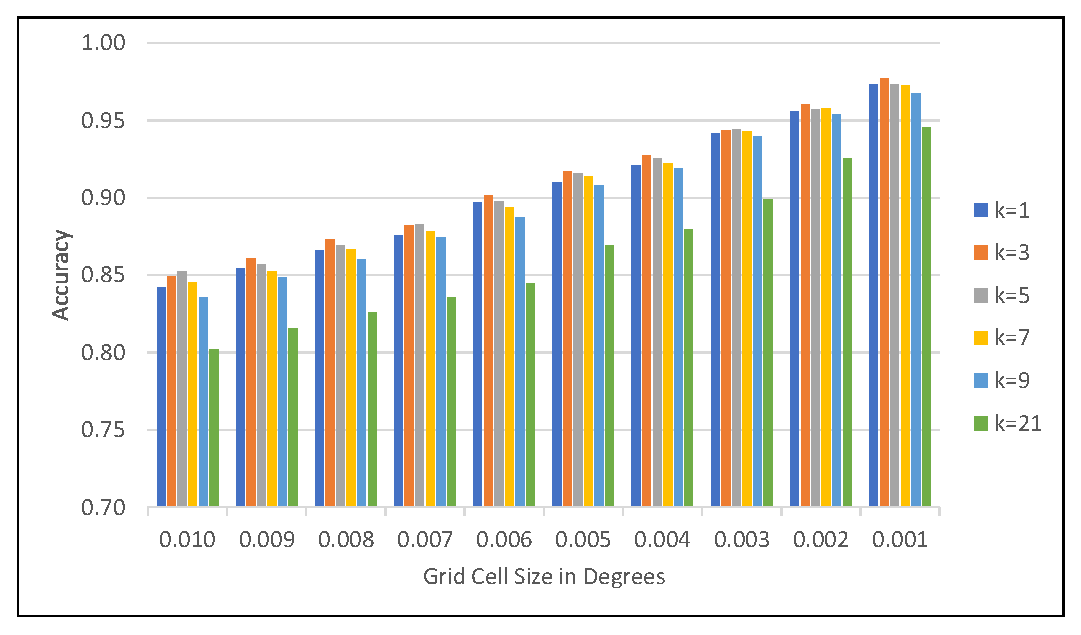
\includegraphics[width = 0.8\textwidth]{figures/jaccard_compare}
		\subcaption{Jaccard Similarity}
    \label{fig:jaccard_compare}
	\end{subfigure}

	\begin{subfigure}[b]{\textwidth}
		\centering
		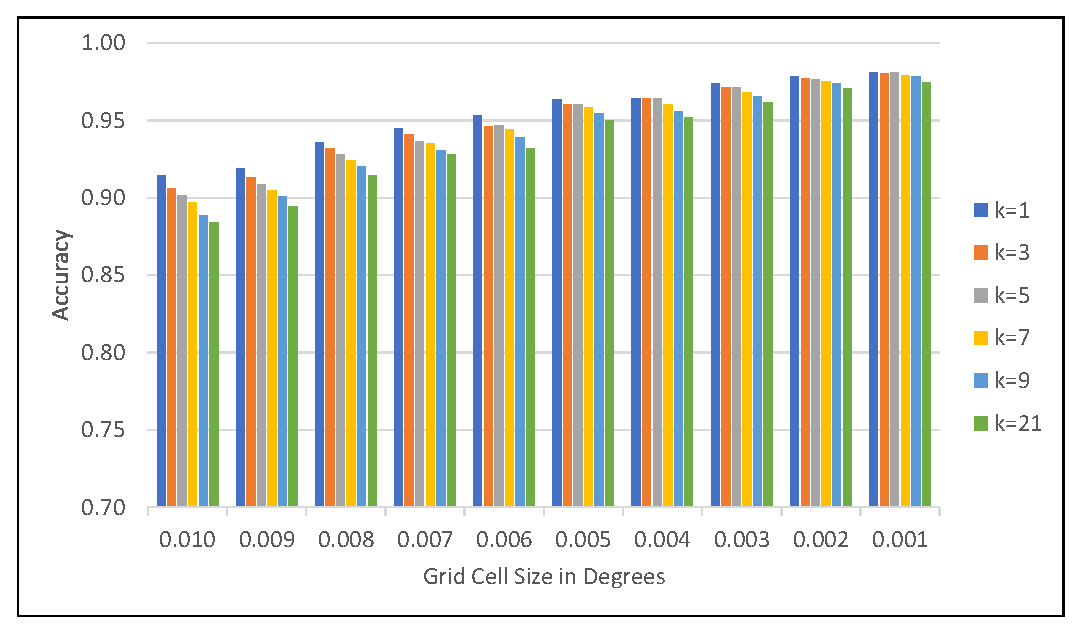
\includegraphics[width = 0.8\textwidth]{figures/cosine_compare}
		\subcaption{Cosine Similarity}
  	\label{fig:cosine_compare}
	\end{subfigure}
  \caption{Classification Accuracy for varying grid-cell size and varying k.}
  \label{fig:results-ext}
	\figSpace
\end{figure}

\section{Accuracy using Set Descriptors}

In the first set of experiments, the accuracy of the user identification is evaluated for different grid-resolutions $ext$, using bitset descriptors for the Jaccard similarity measure (c.f. Definition \ref{subsubsec:set}). The results of this evaluation are shown in Figure \ref{fig:jaccard_compare}. In the basic setting having a relatively coarse spatial grid of $ext=0.01'$, a simple distance weighted $k$NN classification is able to correctly identify up to $85\%$ of individuals for $k=5$. This result improves even further as the grid-resolution $ext$ is increased. In the case of the most detailed grid having $ext=0.001'$, the solution is able to break the $97\%$ classification accuracy line.
This result is quite concerning, as it shows that the motion of individual real-persons is quite characteristic, and that the motion model allows to capture this individuality and allows to discriminate different users very well.

\begin{figure}[tbh]
	\centering
	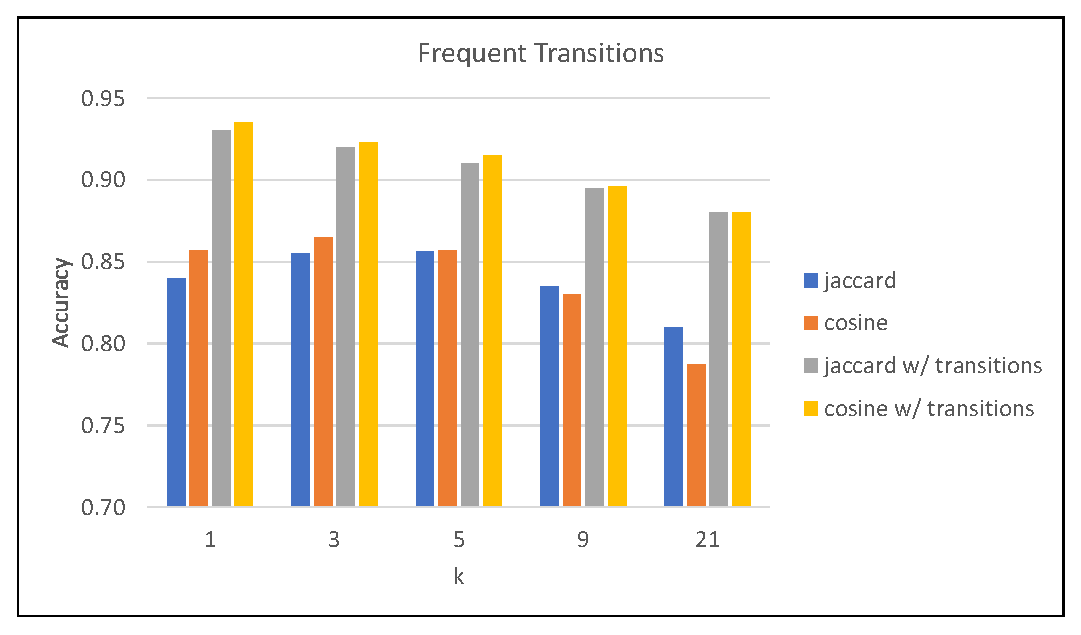
\includegraphics[width = 0.8\textwidth]{figures/topn_transitions}
  \caption{Classification Accuracy using Frequent Transitions.}
  \label{fig:transitions}
	\figSpace
\end{figure}

The classification result are worse for $k=1$ and $k=3$. This result is contributed to chance, as another user may, by chance, have a trajectory very similar to the query trajectory $q_u^e \in Q(u,e)$ of user $u$. However, by using more neighbors, it is likely that the correct user $u$ appears at least twice in the $k=3$ or $k=5$ set, thus out-weighting the erroneous user in the first rank. Yet, for $k>5$ there is a drop in accuracy. This is contributed that the query user only has at most $11$ trajectories in the training set. This number might be less than 11 if a user was not active in all epochs. This is the case for many users, shown by Figure \ref{fig:500_dist}. In the extreme case having $k=21$, at least $10$ trajectories of wrong users must be in the $k$NN result, allowing noise have a much greater effect, especially in the case where $u$ has few trajectories.

Furthermore, Figure \ref{fig:cosine_compare} shows the results using frequency vectors as descriptors, and using the cosine coefficient as a similarity measure (c.f. Definition \ref{subsubsec:set}). The improvement in classification accuracy is relatively minor, but are able to hit the $98\%$ accuracy mark. This result can be contributed to the fact that bitset descriptors already perform so well. Thus, knowing the set of places that a user visited is descriptive enough, such that the frequency of visits does not yield much additional descriptiveness.

\section{Accuracy using Frequent Transitions}

In the next set of experiments, how the usage of transition descriptors (c.f. Section \ref{subsubsec:trans}) instead of set descriptors affects the classification accuracy is evaluated. The results depicted in Figure \ref{fig:transitions} indicate that using from-to-transitions, as opposed to just using sets of cells, further allows to improve the classification quality. An increase in classification accuracy of around $10\%$ (absolute) is observed using transitions, achieving an classification accuracy of nearly $95\%$. This result indicates that the sequence, and thus the motion in space and time is more descriptive than just sets of regions, and thus the motion in space-only.

\section{Accuracy for Different Trajectory Length}
Next, the number of observations required to identify a user accurately is evaluated. Therefore trajectory sizes are created according to the observation distribution in Figure \ref{fig:500_dist}. Then tests are for each trajectory size. If a trajectory does not have the minimum number of observations for the corresponding group, it is not tested, and if a trajectory has more observations than the allowed maximum for the corresponding group, a random sample is taken and tested instead. Thus, instead of testing the accuracy on the original trajectories this tests the accuracy on controlled trajectory sizes.

\begin{figure}[t]
	\centering
	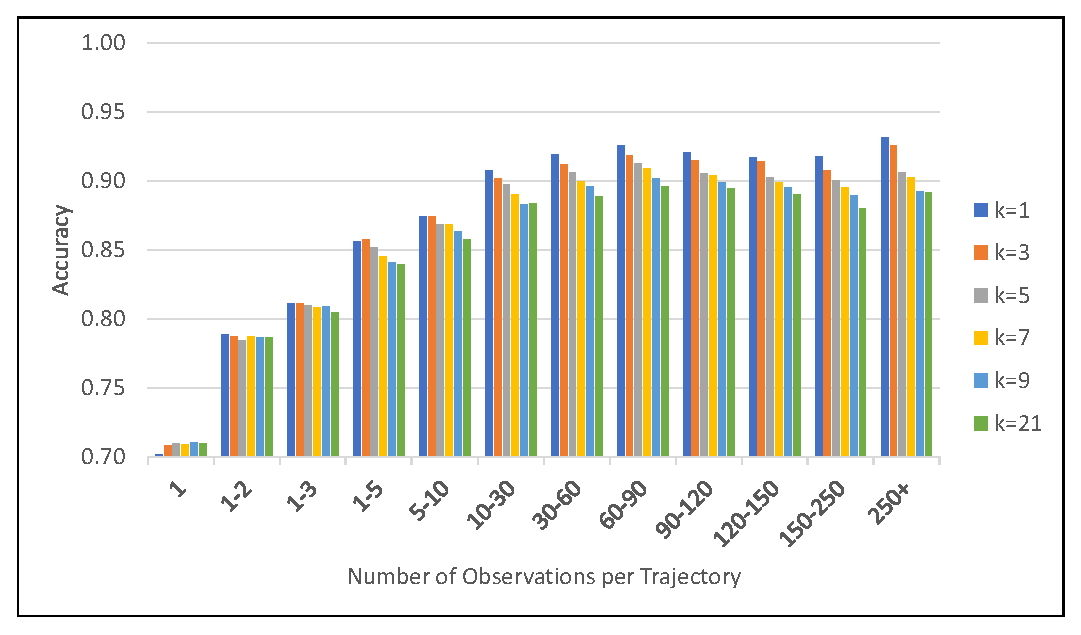
\includegraphics[width = 0.8\textwidth]{figures/archetype_compare}
  \caption{User identification accuracy for different trajectory sizes.}
  \label{fig:archetype}
	\figSpace
\end{figure}

The classification results for each group can be seen in Figure \ref{fig:archetype}. For reference, the set of all trajectories, as used before, is shown first. Surprisingly, in the case of having only one random observation for each trajectory, it is possible to identify over $70\%$ of the users in this dataset. This is likely due to the fact that a random location from a trajectory is likely to pick a users most frequent grid cell, which is most discriminative. Increasing the number of trajectory samples to two, a significant increase in accuracy to $78\%$ is seen, and a steady growth in accuracy from there is shown. Accuracy starts to level off after having 30 or more samples trajectory points from a user. This is surprising, as the vast majority of trajectories has more than 60 observations. Thus, sampling down to 30 observations, yields a significant reduction in data, but as Figure \ref{fig:archetype} shows, yields almost no reduction of discriminative information.

The leveled accuracy level is above $90\%$, which is extremely high for a classification task having 500 different classes. This positive result is also a consequence of large trajectories (i.e., trajectories having a large number of observations) generally having larger trajectories in the training set, as the frequency distribution of tweets among the 500 most prolific Twitter users in London is very skewed. Finally, the classification performs the best, if the parameter of the $kNN$ classification is set to $k=1$. This result is in line with Figure \ref{fig:cosine_compare}, as Cosine-Similarity is used per default in this experiment.

Summarizing this experiment, very short trajectories having $10$ or less observations in space and time are enough to unveil the identity of a user. This is a concerning result.

%!TEX root = ./00_main.tex

\chapter{Scalability}
\label{sec:scalability}

In all of the previous experiments, only the 500 most prolific Twitter users in London were used. In the final experiment, this number of users is scaled up, by using 15,989 users that have a least two trajectories containing at least two observations each. Statistics for this data set are shown in Figure \ref{fig:15989_dist}. The quality of the observed trajectories is  much worse compared to the 500 most prolific users explored in Figure \ref{fig:500_dist}: In Figure \ref{fig:15989_traj} more than half of the trajectories have less than five trajectories within the twelve epochs, and only a small fraction of $6\%$ of the users have maximum number of twelve trajectories. In addition, Figure \ref{fig:15989_obs} shows the quality of these trajectories is much lower, as nearly $50\%$ of the trajectories have three or less observations. Due to the quality of this data a eight-fold split was no longer possible. A stratified shuffle split was used instead, taking 10 iterations of 20\% samples.

\begin{figure}[p]
	\centering
  \begin{subfigure}[b]{\textwidth}
    \centering
    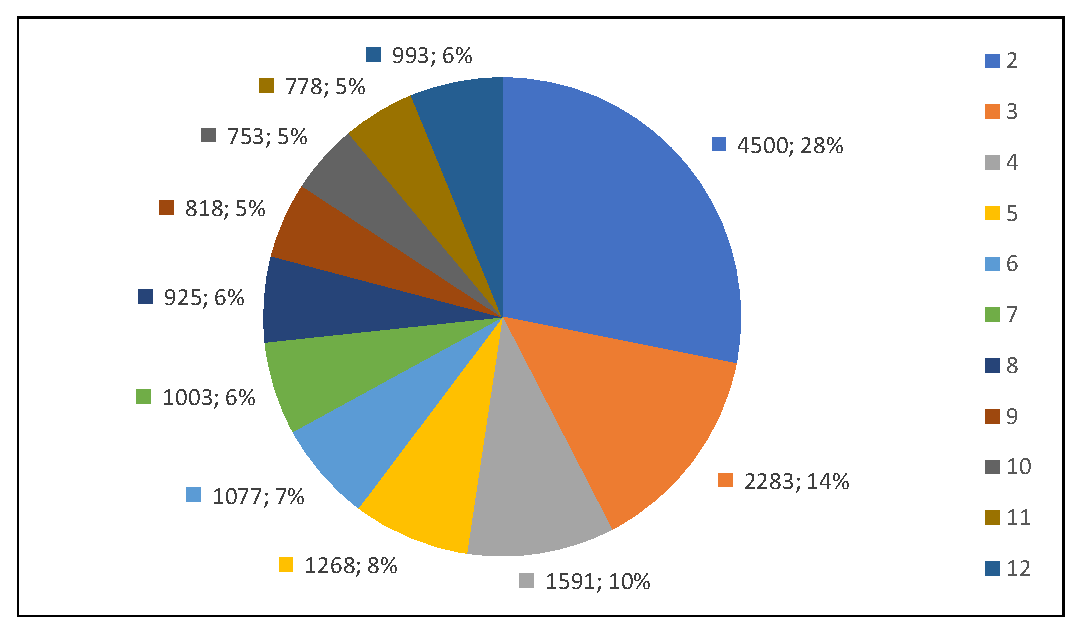
\includegraphics[width = 0.8\textwidth]{figures/15989_trajectories_per_user}
    \subcaption{Trajectories per user.}
    \label{fig:15989_traj}
  \end{subfigure}

  \begin{subfigure}[b]{\textwidth}
    \centering
    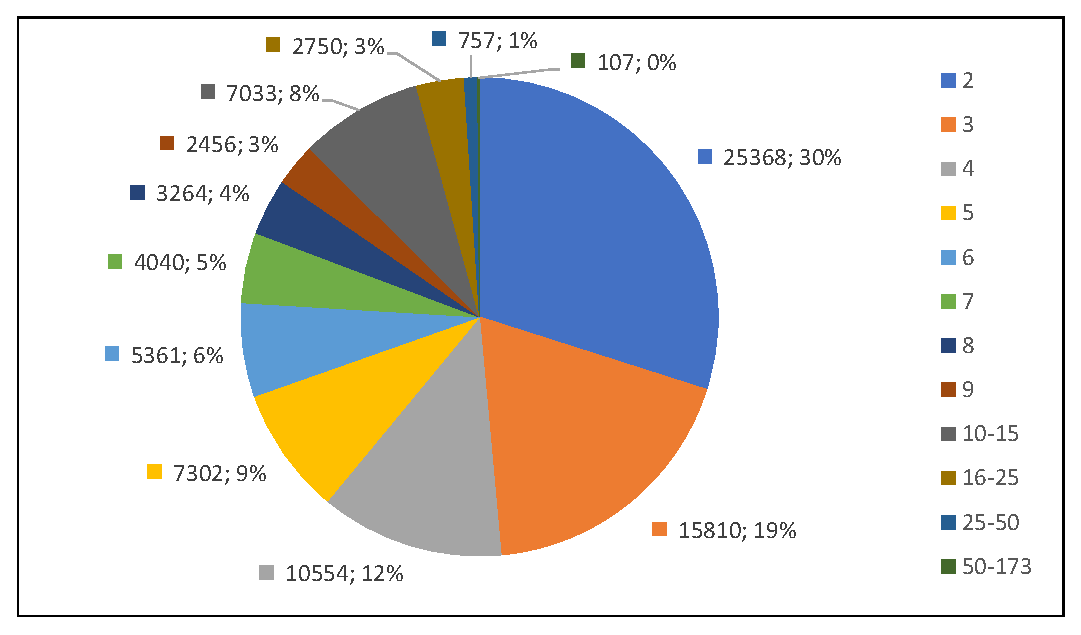
\includegraphics[width = 0.8\textwidth]{figures/15989_observations_per_trajectory}
  	\subcaption{Observations per one-week Trajectory}
    \label{fig:15989_obs}
  \end{subfigure}
  \caption{Distribution of all 15,989 users in the London-Twitter Dataset.}
  \label{fig:15989_dist}
	\figSpace
\end{figure}

The results on this data set, in terms of classification accuracy as well as run-times are shown in Figure \ref{fig:scalability_results}. In terms of accuracy, there is a vast decrease in accuracy observed, even for the default setting of $500$ users. This is because the experiments are no longer using the most prolific users, but just a random sample of users, and the data quality, in terms of number of observations per trajectory, as well as the number of trajectories per user, is much lower for these users.

\begin{figure}[p]
	\centering
  \begin{subfigure}[b]{\textwidth}
    \centering
    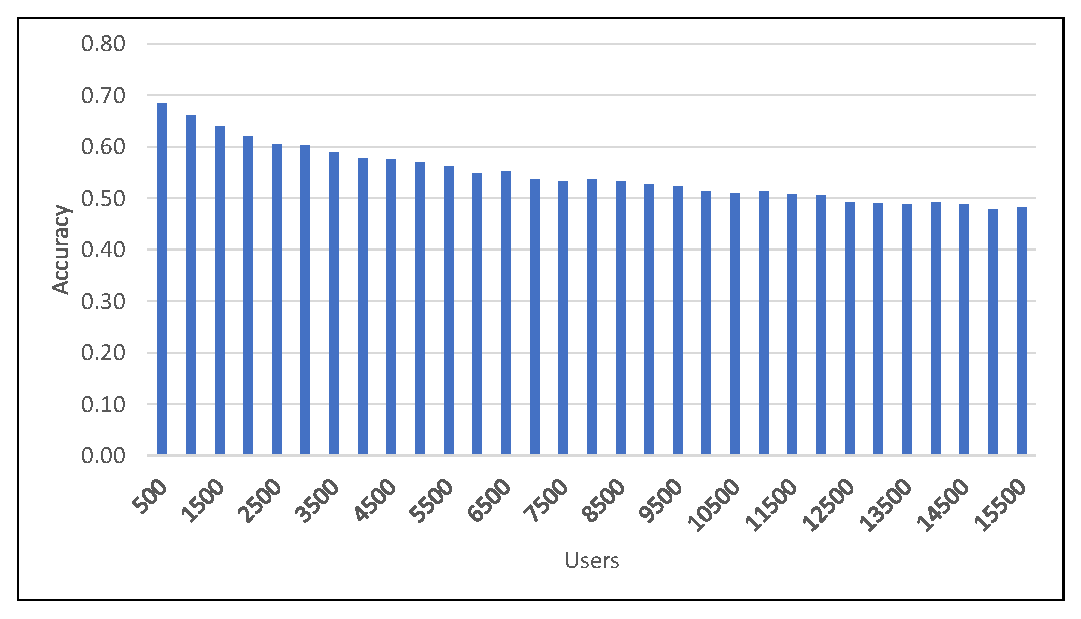
\includegraphics[width = 0.8\columnwidth]{figures/scalability_accuracy}
    \subcaption{Classification Accuracy}
    \label{fig:scalability_accuracy}
  \end{subfigure}

  \begin{subfigure}[b]{\textwidth}
    \centering
    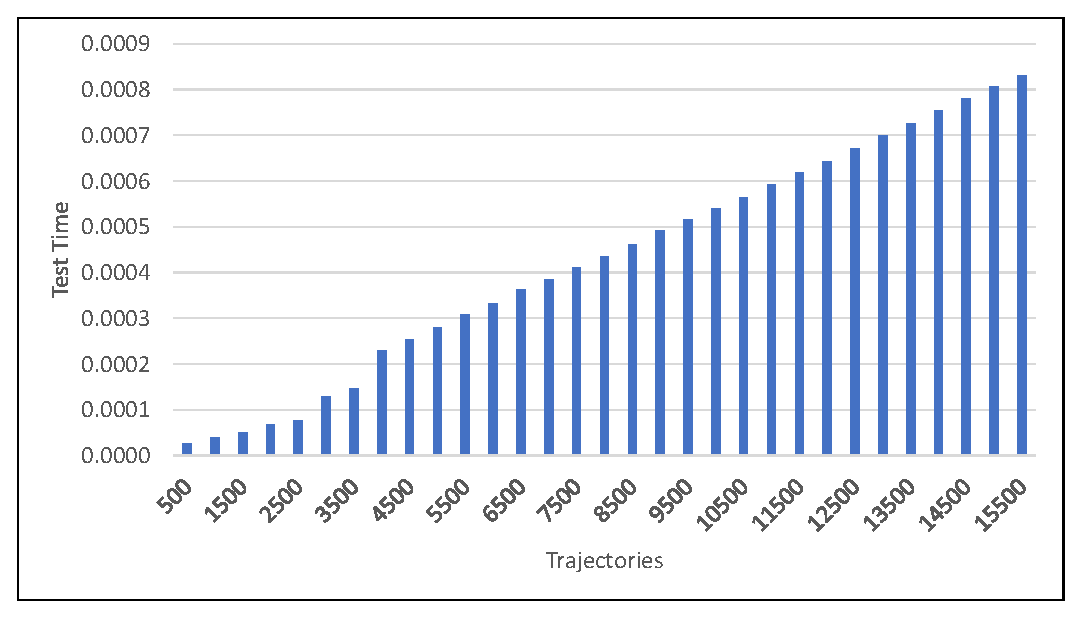
\includegraphics[width = 0.8\columnwidth]{figures/scalability_runtime}
    \subcaption{Run-time (in seconds)}
    \label{fig:scalability_runtime}
  \end{subfigure}
  \caption{Scalability: Scaling the number of Twitter users.}
  \label{fig:scalability_results}
	\figSpace
\end{figure}

Clearly, less prolific users are harder to classify, since there is less information. As the experiments are scaled up the number of users, there is a decrease in classification accuracy, as the classification problem becomes harder having more users. Still, the classification accuracy remains at almost $50\%$, despite the large number of  15,989 users, and the much lower trajectory quality.

Since a $k$NN classification is employed, and thus a lazy learning method is used, there is no model learning phase. The run-time results for the classification is shown in Figure \ref{fig:scalability_runtime}.\footnote{Run-time tests were performed on AWS using a m4.2xlarge EC2 instance running Amazon Linux. This instance type has 8 CPU cores and 32GB of RAM.} a linear run-time is observed, which is attributed to the extreme high dimensionality of the feature vectors, which cannot be beneficially supported by an index structure for the $k$NN search. But even at the full 15,989 users, the time to classify each trajectory is less than $1ms$.

%!TEX root = ./00_main.tex

\chapter{User Linkage between different Social Networks}
\label{sec:linkage}

In all the previous experiments, a single user had to be identified based on a new trajectory. In this section, the next step is evaluated, of linking whole sets of users of two different social networks, based on their trajectories, as described in Section \ref{subsec:linkage}. For this purpose, two data sets are employed, one generated synthetically from the Twitter data set, and one using authoritative ground-truth links between Twitter and Instagram.

\begin{figure}[p]
	\centering
  \begin{subfigure}[b]{\textwidth}
    \centering
    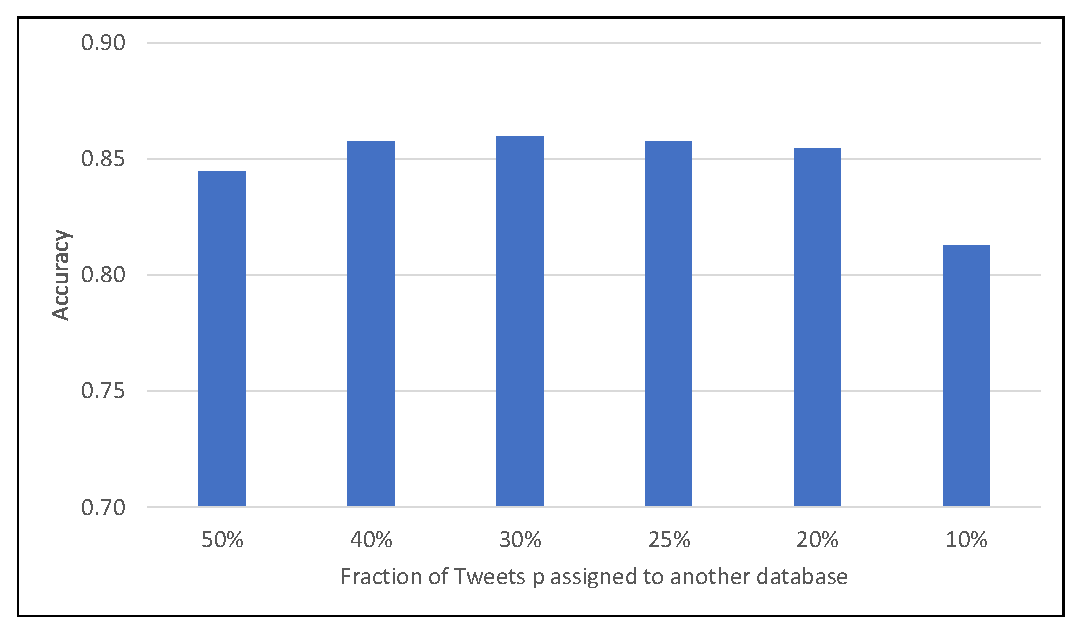
\includegraphics[width = 0.8\textwidth]{figures/sample_accuracy}
    \subcaption{User Linkage results for different fractions of user belonging to each database.}
    \label{fig:split_test}
  \end{subfigure}

  \begin{subfigure}[b]{\textwidth}
		\centering
    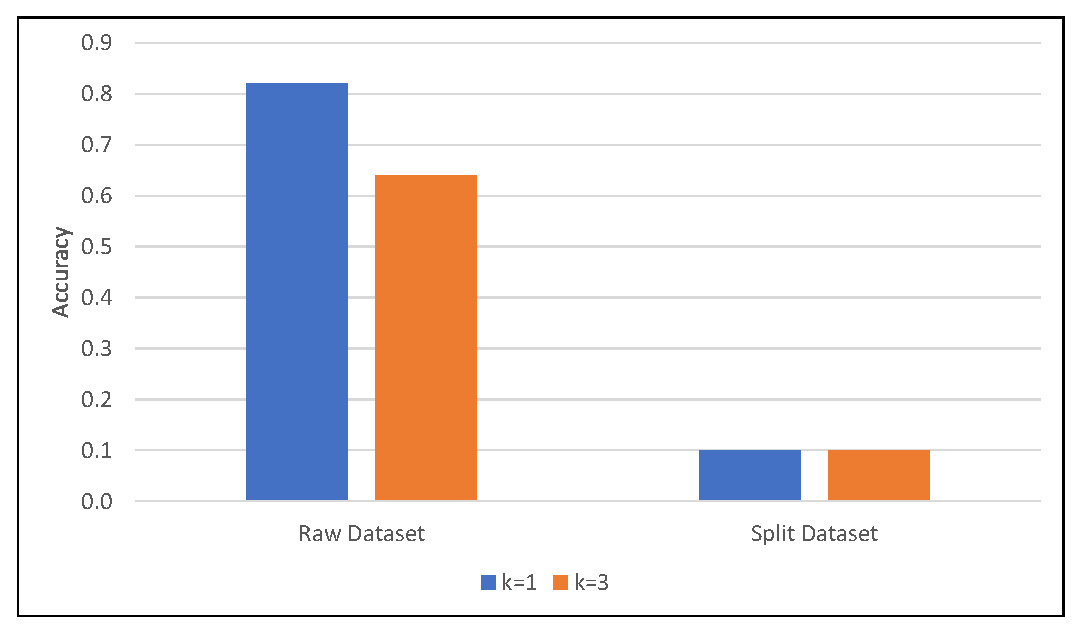
\includegraphics[width = 0.8\textwidth]{figures/split_accuracy}
    \subcaption{User Linkage results for linking Twitter and Instagram.}
    \label{fig:instagram}
  \end{subfigure}
  \caption{Classification Accuracy for different Social Networks.}
  \label{fig:split-results-ext}
	\figSpace
\end{figure}

{\bf Synthetic Database Split:} For the synthetic database, a fraction of $p$ Tweets is uniformly sampled from the Twitter dataset $\DB$, and pretend that this set belongs to a different social network $\DB^\prime$. In this sampled database $\DB^\prime$, the user-labels as ground-truth, which the algorithm tries to predict given the data in $\DB$ can be used. For this experiment, only trajectories having at least 10 tweets to sample from are considered. If uniform sampling of a trajectory yields an empty set, it is re-sampled.

{\bf Instagram Data:} Out of the 2.7 million tweets in the dataset, a significant portion of 204 thousand tweets is labelled as coming from the Instagram network. These Tweets were cross posted by the user, on both Instagram and Twitter. Thus, the Instagram database $\DB^I$ consists of all these cross-linked posts. For the Twitter database, two cases are evaluated. In the first case, the full dataset $\DB$ can simply be used, thus assuming that the Instagram observations were made in both datasets. In the second case, the database $\DB_T=\DB\setminus \DB_I$ is used, thus assuming that the Instagram observations were made in the Instagram network only.

The results on the synthetic database split are shown in Figure \ref{fig:split_test}.
For each value of $p$, 10 random samples of the database $\DB$ are obtained, and averaged the results in order to avoid effects generated due to random sampled. In all ten runs, the depicted values showed almost no deviation, all being in a $\pm 0.5\%$ interval. An even 50/50 split yields a correct linkage rate of almost $85\%$. Yet, this split becomes biased towards a smaller value $p$. This can be explained by having a larger sample in the training database $\DB$, on which the trajectories of $\DB^\prime$ are queried on. However, for $p=0.1$, this accuracy drops significantly. This can be explained by the previous experiments, showing that a sample of as little as three observations suffices for a high classification accuracy. However, since many of the trajectories only have $10-20$ observations, there is a high chance that a $10\%$ random sample may only have one or two observations.

For the Instagram-Twitter matching, the results are shown in Figure \ref{fig:instagram}, for the two cases of using the data as is, thus having all Instagram observations also present in the Twitter database, and the case of splitting the dataset, thus removing the Instagram observations from the Twitter trajectories. Using the raw dataset a prediction accuracy of roughly $80\%$ using $k=1$ nearest neighbor classification to build the bi-partite graph is observed.

In contrast, the case of splitting Instagram off of Twitter, the accuracy drops to about $10\%$. These disappointing results can be explained by making the hypothesis that users use Instagram and Twitter in different ways, such as using Instagram when on a far-away vacation, while also using Twitter in locations where you don't usually take a picture, such as work and home. Also, some of the users had all their tweets linked to Instagram, such that the algorithm had no training data left in the Twitter database, thus having to random guess the user. Thus, it appears that Twitter and Instagram are used differently by users, making the Instagram sample much harder to match than a uniform random sample taken from Twitter.

%!TEX root = ./00_main.tex

\chapter[Conclusion]{Conclusion}
\label{sec:conclusion}
In this work, the challenge of identifying users in a spatio-temporal database was approached. This approach uses historic trajectories of a user to learn their motion in space and time, by proposing various feature extraction and similarity search methods. Using a 12-week dataset of Tweets in the London region, the experimental results show that it is possible to map a trajectory to a ground-truth user with extremely high accuracy. This raises various concerns and opportunities:
\begin{itemize}
  \item {\bf The Threat} of loss of privacy: Trajectories of real people are publicly available. Given only few observations of an individual. For example, one person inadvertently appearing in the background of another person's Facebook images, then identifying this user in a trajectory database, and linking them to additional data, such as username or real name.
  \item {\bf The Potential} through record linkage of trajectory databases. For example, joining the personal interests in locations (such as restaurants, bars, cafes) from a LBSN with textual thoughts of a user from a micro-blog. Thus, a micro-blog tweet from user $u$ such as {\bf ``W00T, I'm going to George Mason University!''}, might be used to recommend restaurants to $u$ by mining their restaurant preferences using their check-ins in the LBSN.
  \item {\bf The Challenge} of privacy preservation by trajectory obfuscation and other means. By learning the characteristics that make a trajectory matchable to its user, techniques to hide particularly descriptive and discriminative observations from the public trajectory can be developed.
\end{itemize}

%!TEX root = ./00_main.tex

\chapter[Additional Research Opportunities]{Additional Research Opportunities}
\label{sec:additional}

There are many additional research opportunities that could follow on this work, in a wide area of topics. Some of those areas might include:

\begin{itemize}
  \item Utilizing this research with addition sources of trajectories to further validate the work in it. A prime target for this would be using twitter and Instagram data to link users across multiple platforms.
  \item Additional research into frequent transitions. This research showed the sequence of locations a user visits can add additional uniqueness, allowing users to be identified more easily, however there is likely room for improvement. The transitions added additions dimensionality to an problem, which was already extremely dimensional, and was not a primary focus of this research.
  \item Dimension reduction, or some form of principle component analysis, could provide significant improvements to this research. The dimensionality of the data will likely cause issues when scaling up to a larger area of interest, and could become a hindrance in very large areas.
  \item A tiered approach could be useful for larger areas of interest, to include world wide analysis. One might be able to use a very coarse grid at a world scale, in order to group users together into smaller areas. Then they could keep drilling down into smaller and smaller areas. At each level, there may be a set of unique users, which are identifiable, and the rest can be drilled down on at a finer scale.
\end{itemize}


%%
%%  bibliography
%%

%% list all of the BibTeX files here for the WinEdt project (if applicable)
%GATHER{bibfile.bib}

%% any bibliography style can be used, but IEEEtran.bst is ideally suited to
%% electrical engineering references

%% include the following directives if there are any appendices
\appendix
\appendixeqnumbering
% !TeX root = 00_main.tex

% N.B.: an appendix chapter starts with "appchapter" instead of "chapter"
%
% The first argument in [ ] is the title as displayed in the table of contents
% The second argument is the title as displayed here.  Use \\ as appropriate in
%   this title to get desired line breaks
\appchapter[Metric Accuracies]{Metric Accuracies}

The following tables include the accuracies for all metrics attempted, on the 500 user dataset, in order to discern which would be the best to start with in the experiments of this work. This was an exhaustive search of all possible combinations offered within scikit-learn \cite{scikit-learn}.


\begin{table}
  \centering
  \caption{Accuracy for all Metrics (k = 1)}
  \begin{tabular}{|l|l|l|l|}
    \hline
    {\bf Metric} & {\bf Index} & {\bf Accuracy} & {\bf Std. Dev.} \\\hline
    euclidean & kd tree & 0.838188 & 0.044796 \\\hline
    manhattan & kd tree & 0.826809 & 0.057972 \\\hline
    chebyshev & kd tree & 0.820695 & 0.039398 \\\hline
    euclidean & ball tree & 0.837978 & 0.044938 \\\hline
    manhattan & ball tree & 0.827230 & 0.058734 \\\hline
    chebyshev & ball tree & 0.820695 & 0.038600 \\\hline
    hamming & ball tree & 0.466513 & 0.052677 \\\hline
    canberra & ball tree & 0.723581 & 0.086002 \\\hline
    braycurtis & ball tree & 0.891077 & 0.044141 \\\hline
    jaccard & ball tree & 0.840933 & 0.054737 \\\hline
    dice & ball tree & 0.840933 & 0.054737 \\\hline
    kulsinski & ball tree & 0.751595 & 0.063372 \\\hline
    rogerstanimoto & ball tree & 0.731370 & 0.061987 \\\hline
    russellrao & ball tree & 0.625803 & 0.074475 \\\hline
    sokalmichener & ball tree & 0.731370 & 0.061987 \\\hline
    sokalsneath & ball tree & 0.840933 & 0.054737 \\\hline
    euclidean & brute & 0.838188 & 0.044796 \\\hline
    manhattan & brute & 0.827019 & 0.058927 \\\hline
    chebyshev & brute & 0.820274 & 0.038897 \\\hline
    hamming & brute & 0.462506 & 0.048503 \\\hline
    canberra & brute & 0.723791 & 0.086601 \\\hline
    braycurtis & brute & 0.891077 & 0.044141 \\\hline
    jaccard & brute & 0.342842 & 0.101260 \\\hline
    dice & brute & 0.840933 & 0.055508 \\\hline
    kulsinski & brute & 0.751595 & 0.064149 \\\hline
    rogerstanimoto & brute & 0.729263 & 0.064473 \\\hline
    russellrao & brute & 0.622429 & 0.071010 \\\hline
    sokalmichener & brute & 0.729263 & 0.064473 \\\hline
    sokalsneath & brute & 0.840933 & 0.055508 \\\hline
    cosine & brute & 0.914248 & 0.029629 \\\hline
  \end{tabular}
  \tableSpace
\end{table}

\begin{table}
  \centering
  \caption{Accuracy for all Metrics (k = 3)}
  \begin{tabular}{|l|l|l|l|}
    \hline
    {\bf Metric} & {\bf Index} & {\bf Accuracy} & {\bf Std. Dev.} \\\hline
    euclidean & kd tree & 0.827866 & 0.053549 \\\hline
    manhattan & kd tree & 0.817327 & 0.062069 \\\hline
    chebyshev & kd tree & 0.813746 & 0.042208 \\\hline
    euclidean & ball tree & 0.827866 & 0.053549 \\\hline
    manhattan & ball tree & 0.818170 & 0.062555 \\\hline
    chebyshev & ball tree & 0.813957 & 0.041596 \\\hline
    hamming & ball tree & 0.464402 & 0.049754 \\\hline
    canberra & ball tree & 0.710095 & 0.081823 \\\hline
    braycurtis & ball tree & 0.885812 & 0.046944 \\\hline
    jaccard & ball tree & 0.849785 & 0.065483 \\\hline
    dice & ball tree & 0.850628 & 0.065584 \\\hline
    kulsinski & ball tree & 0.765713 & 0.059737 \\\hline
    rogerstanimoto & ball tree & 0.717679 & 0.072936 \\\hline
    russellrao & ball tree & 0.633812 & 0.067216 \\\hline
    sokalmichener & ball tree & 0.717679 & 0.072936 \\\hline
    sokalsneath & ball tree & 0.849363 & 0.064541 \\\hline
    euclidean & brute & 0.827866 & 0.053549 \\\hline
    manhattan & brute & 0.818170 & 0.061136 \\\hline
    chebyshev & brute & 0.814378 & 0.040797 \\\hline
    hamming & brute & 0.459136 & 0.055243 \\\hline
    canberra & brute & 0.709674 & 0.081047 \\\hline
    braycurtis & brute & 0.885812 & 0.046944 \\\hline
    jaccard & brute & 0.349590 & 0.107582 \\\hline
    dice & brute & 0.849995 & 0.065003 \\\hline
    kulsinski & brute & 0.765502 & 0.060497 \\\hline
    rogerstanimoto & brute & 0.717048 & 0.076714 \\\hline
    russellrao & brute & 0.630017 & 0.065846 \\\hline
    sokalmichener & brute & 0.717048 & 0.076714 \\\hline
    sokalsneath & brute & 0.848731 & 0.064078 \\\hline
    cosine & brute & 0.906244 & 0.039755 \\\hline
  \end{tabular}
  \tableSpace
\end{table}

\begin{table}
  \centering
  \caption{Accuracy for all Metrics (k = 5)}
  \begin{tabular}{|l|l|l|l|}
    \hline
    {\bf Metric} & {\bf Index} & {\bf Accuracy} & {\bf Std. Dev.} \\\hline
    euclidean & kd tree & 0.824074 & 0.055560 \\\hline
    manhattan & kd tree & 0.815642 & 0.061258 \\\hline
    chebyshev & kd tree & 0.811429 & 0.045801 \\\hline
    euclidean & ball tree & 0.824074 & 0.055560 \\\hline
    manhattan & ball tree & 0.816696 & 0.062219 \\\hline
    chebyshev & ball tree & 0.811219 & 0.046123 \\\hline
    hamming & ball tree & 0.460613 & 0.055359 \\\hline
    canberra & ball tree & 0.690076 & 0.067420 \\\hline
    braycurtis & ball tree & 0.887290 & 0.053699 \\\hline
    jaccard & ball tree & 0.852103 & 0.064630 \\\hline
    dice & ball tree & 0.854210 & 0.061707 \\\hline
    kulsinski & ball tree & 0.764875 & 0.073723 \\\hline
    rogerstanimoto & ball tree & 0.702083 & 0.064854 \\\hline
    russellrao & ball tree & 0.660578 & 0.072486 \\\hline
    sokalmichener & ball tree & 0.702083 & 0.064854 \\\hline
    sokalsneath & ball tree & 0.851261 & 0.064230 \\\hline
    euclidean & brute & 0.823231 & 0.054043 \\\hline
    manhattan & brute & 0.814588 & 0.060960 \\\hline
    chebyshev & brute & 0.810586 & 0.045200 \\\hline
    hamming & brute & 0.463354 & 0.063333 \\\hline
    canberra & brute & 0.691129 & 0.065973 \\\hline
    braycurtis & brute & 0.887079 & 0.053926 \\\hline
    jaccard & brute & 0.350008 & 0.099094 \\\hline
    dice & brute & 0.854842 & 0.062671 \\\hline
    kulsinski & brute & 0.765295 & 0.071434 \\\hline
    rogerstanimoto & brute & 0.701664 & 0.069232 \\\hline
    russellrao & brute & 0.636137 & 0.072479 \\\hline
    sokalmichener & brute & 0.701664 & 0.069232 \\\hline
    sokalsneath & brute & 0.852525 & 0.066063 \\\hline
    cosine & brute & 0.901398 & 0.034491 \\\hline
  \end{tabular}
  \tableSpace
\end{table}

% !TeX root = 00_main.tex

% Additional chapter
\appchapter[Source Code]{Source Code}

All code for this document, and the experiments described in it, is available at:

\url{https://github.com/eseglem/thesis}


\bibliographystyle{IEEEtranN}
\bibliography{bibfile}

%%
%% curriculum vitae
%%
\cvpage

\noindent
Erik L. Seglem will soon to be a PhD. student in the Earth Systems and Geoinformation Sciences program. He received a Bachelors of Arts in Intelligence Studies from American Military University in August of 2014, and is graduating from George Mason University with a Master’s of Science in Geoinformatics and Geospatial Intelligence.  In November of 2016 he won First Place in the Graduate category of the Student Research Poster Competition at GMU’s GIS Day. With over 9 years of experience in GIS, including 5 years in the Marine Corps as a Geospatial Analyst, and 4 years as a Geospatial Software Engineer at DigitalGlobe Inc. He has taken a new position at BigBear Inc, where he will be focusing on cloud technology and big data as it applies to geospatial problems.

\end{document}
